Energy landscapes can describe an incredible array of systems, particularly biological and chemical processes.
% Cite Nature article as well as related research
It is therefore vital to understand the stable states in this system, and the transitions between them.
% https://chem.libretexts.org/Bookshelves/Physical_and_Theoretical_Chemistry_Textbook_Maps/Supplemental_Modules_(Physical_and_Theoretical_Chemistry)/Kinetics/Modeling_Reaction_Kinetics/Temperature_Dependence_of_Reaction_Rates/The_Arrhenius_Law/The_Arrhenius_Law%3A_Activation_Energies
% http://www.math.uni-leipzig.de/~quapp/wqTCA84.pdf
For example, if you can find the transition pathway between two stable states in a chemical reaction that has the lowest possible maximum energy then it is possible to deduce information about reaction speed.
Such a pathway is called the minimum energy pathway.

A significant amount of research has been devoted to finding these minimum energy pathways.
A popular method is called Nudged Elastic Band (NEB), which lets the path be a string of points.
It starts with a random guess (normally a straight line between two stable points), and then lets the points fall down the slope of the energy landscape (given by the gradient of the energy function).
% Cite algorithm used
However it then forces the points to remain equidistant by exerting a spring force on them\footnote{This is a slight simplification, as moderations are made to stop the algorithm cutting corners. See the paper cited for implementation details.}.

This algorithm is a form of gradient descent.
As with any form of gradient descent the algorithm can get stuck in local minima, as in Figure~\ref{fig:global_local_min}.
When the gradient descent is run the path gets stuck in a high energy valley, when going around gives a lower energy result.

\begin{figure}[h]
    \centering
    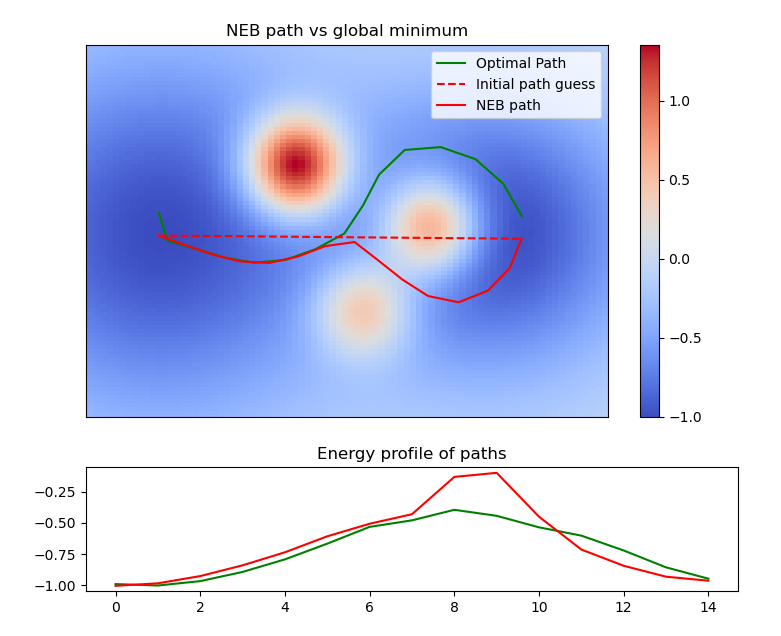
\includegraphics[width=10cm]{possible paths.png}
    \caption{The NEB generated and global minimum energy path between two minima (above) with the energy profile of those paths (below).}
    \label{fig:global_local_min}
\end{figure}

In this paper we propose an algorithm that can efficiently explore the landscape and the possible paths.
This algorithm is therefore able to find very promising initial path guesses that outperform naive NEB, and it even has the ability to quickly find a selection of paths that go through different areas of the energy landscape.
We provide an analysis of how this algorithm performs in different situations - including the time it takes to run as well as the quality of the outputted paths.
%cite pls
We will refer to this algorithm as the Max-Product Message Passing (MPMP) algorithm.
This is because MPMP is the main part of the algorithm that does the calculations to work out the best paths.
However, in some charts the process may be referred to as Markov Random Field (MRF), which is closely related to MPMP\@.

\section{Basic MRF algorithm description}
\label{sec:basic_algo}
The algorithm effectively defines the path by a number of points.
It works along the path step by step, testing a number of positions for each point and working out the how good that possible position is.
When working out the quality of a position it incorporates the quality of all the points leading up to that position using an algorithm called max-produce message passing.
If effectively scans the points that lead up to each position and picks the preceeding path that maximises its quality.

Once we have found the path we then smooth out the generated path with the Nudged Elastic Band method, as if our suggested path is close to the minimum path then NEB should converge to it.
This is important since the algorithm must perform a very coarse scan of the landscape for time complexity reasons.
The algorithm scales linearly by the number of positions being scanned, multiplied by the number of positions on average that one position is connected to.
This means that particularly in high dimensions, with a lot of space that you need to explore, the produced path cannot be very fine grained.

This method leaves us with a few important questions, which we will consider in the paper:
\begin{itemize}
    \item How do we decide the possible positions and transitions that our path could go through?
    \item How do we define the quality of a point or a transition?
    \item How do we make it all fit together?
    \item How long does this algorithm take to run?
    How does this compare to NEB?
    \item What are the other possible algorithms that might be able to do this?
    \item Are the outputs of this algorithm better than naive NEB?
\end{itemize}